% Asset ID: FA21ConicSections2EnrichmentTikZ-002
% Source: vertical ellipse foci/directrices example
% Boundary status: Off-spec enrichment until official CCEA conics evidence is supplied.
\documentclass[tikz,border=8pt]{standalone}
\usepackage{amsmath,amssymb}
\usetikzlibrary{arrows.meta,calc,positioning}
\definecolor{Canvas}{HTML}{FAF9F6}
\definecolor{Ink}{HTML}{2C2C2E}
\definecolor{Gold}{HTML}{C5A059}
\definecolor{GoldDeep}{HTML}{D4AF37}
\begin{document}
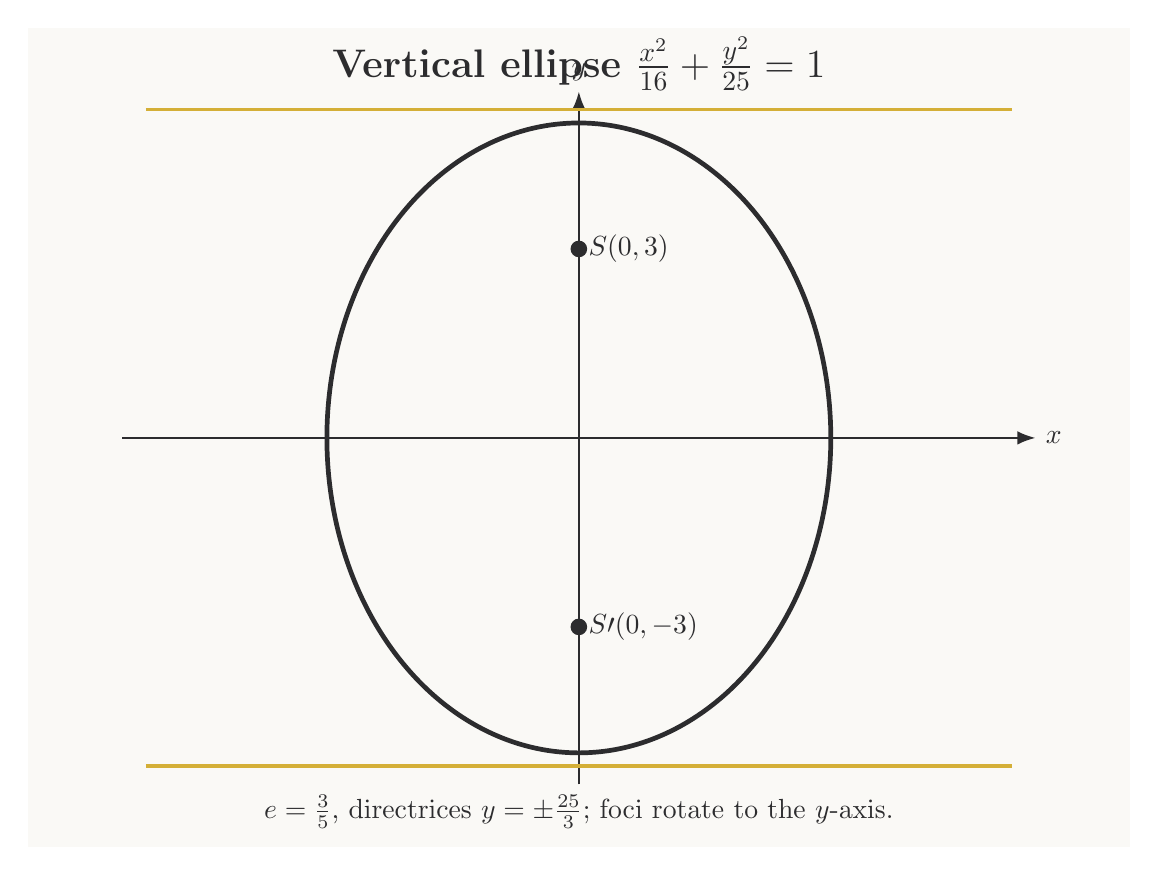
\begin{tikzpicture}[x=1cm,y=1cm,>=Latex]
\fill[Canvas] (-7,-5.2) rectangle (7,5.2);
\node[Ink, font=\Large\bfseries] at (0,4.75) {Vertical ellipse $\frac{x^2}{16}+\frac{y^2}{25}=1$};
\draw[Ink, thick, -Latex] (-5.8,0)--(5.8,0) node[right] {$x$};\draw[Ink, thick, -Latex] (0,-4.4)--(0,4.4) node[above] {$y$};\draw[GoldDeep, very thick] (-5.5,{25/6}) -- (5.5,{25/6});\draw[GoldDeep, very thick] (-5.5,{-25/6}) -- (5.5,{-25/6});\draw[Ink, line width=1.7pt, smooth, samples=240, domain=0:360, variable=\t] plot ({3.2*cos(\t)}, {4*sin(\t)});\fill[Ink] (0,2.4) circle (3pt) node[right] {$S(0,3)$};\fill[Ink] (0,-2.4) circle (3pt) node[right] {$S\prime(0,-3)$};\node[Ink] at (0,-4.75) {$e=\frac35$, directrices $y=\pm\frac{25}{3}$; foci rotate to the $y$-axis.};
\end{tikzpicture}
\end{document}
